\documentclass[a4j,titlepage]{jsarticle}

\usepackage[dvipdfmx]{graphicx,xcolor}
\usepackage[top=20truemm,left=25truemm,right=25truemm]{geometry}
\usepackage{amsmath}
\usepackage{here}
\usepackage{comment}
\usepackage{url}
\usepackage{plistings}
\usepackage{tikz}
\usepackage[framemethod=tikz]{mdframed}

\renewcommand{\lstlistingname}{リスト}

\newcommand{\chuo}[1]{\multicolumn{1}{|c|}{#1}}
\newcommand{\inpt}[1]{\underline{#1}\,\setlength{\fboxsep}{1pt}\fbox{\small ↓}}

\lstdefinestyle{C}{
  language=C,
  basicstyle=\small\ttfamily,
  keywordstyle=\color[HTML]{0000E0},
  stringstyle=\color[HTML]{A31515},
  commentstyle=\upshape\color[HTML]{008000},
  frame=trbl,
  framesep=5pt,
  columns=[l]{fullflexible},
  numbers=left,
  xleftmargin=3zw,
  lineskip=-0.2ex,
  breaklines=true,
  showstringspaces=false,
  tabsize=4,
  keepspaces=true
}

\lstdefinestyle{make}{
  language=,
  basicstyle=\small\ttfamily,
  keywordstyle=\color[HTML]{0000E0},
  stringstyle=\color[HTML]{A31515},
  commentstyle=\upshape\color[HTML]{008000},
  frame=trbl,
  framesep=5pt,
  columns=[l]{fullflexible},
  numbers=left,
  xleftmargin=3zw,
  lineskip=-0.2ex,
  breaklines=true,
  showstringspaces=false,
  tabsize=4,
  keepspaces=true
}

\lstdefinestyle{text}{
  language=,
  basicstyle=\ttfamily,
  frame=trbl,
  framesep=5pt,
  columns=[l]{fullflexible},
  xleftmargin=3zw,
  lineskip=-0.2ex,
  showstringspaces=false,
  tabsize=4,
  keepspaces=true
}

\mdfsetup{
  skipabove=5pt,
  innertopmargin=10pt,
  innerbottommargin=10pt,
  roundcorner=10pt,
  font=\ttfamily
}


\begin{document}


\begin{titlepage}
  \title{\huge{プログラミング演習} \\ \LARGE{---アナログ時計---}}
	\author{学籍番号:16426 \\ 4年 電子情報工学科 23番 \\ 福澤 大地}
	\date{提出日 : 2019年12月9日}
  \maketitle
\end{titlepage}


\section{目的}
OpenGL (Open Graphics Library)に準拠したC言語のライブラリ``GLUT (OpenGL Utility Toolkit)''
を用いてアナログ時計のプログラムを作成することで、
グラフィカルなウィンドウアプリケーションを作成できるようになる。
また、コールバック関数を用いたイベント駆動型プログラミングを行うことで、
インタラクティブなユーザーインターフェースを実現する。


\section{作成したアナログ時計}
内部の歯車や振り子が透けて見えるような振り子時計を作成した。
歯車や振り子などのパーツはGLUTの関数を用いて描画し、
時間変化に応じて現実の時計と同じような仕組みで動作する。

また、ウィンドウのサイズを変更したときに自動的に時計の大きさが変わり、
ウィンドウの領域を最大限に利用して表示されるような機能も実装した。


\section{開発環境}
プログラムの開発、実行を行った環境を表\ref{tb:kan}に示す。

\begin{table}[H]
  \centering
  \caption{開発環境}
  \label{tb:kan}

  \begin{tabular}{|l|l|}
    \hline
    CPU & Intel Core i5-7400 @ 3.0GHz \\ \hline
    メモリ & 8GB \\ \hline
    OS & Microsoft Windows 10 Home \\ \hline
    システム & 64bit \\ \hline
    実行環境 & Cygwin 3.0.7 \\ \hline
    コンパイラ & GCC 7.4.0 \\ \hline
    OpenGLライブラリ & GLUT 3.7 \\ \hline
  \end{tabular}
\end{table}


\section{OpenGLとGLUT \cite{bib:1}}
OpenGLとは、2次元/3次元のコンピュータグラフィックライブラリである。
幅広い処理系に対応しており、汎用性が高いため、広く普及している。

一方で、簡素な機能しか用意されていない分複雑な処理は向いていないため、
それを補うために登場したのがGLU (OpenGL Utility Library)である。
GLUはOpenGLの補助的なライブラリであり、円柱などの複雑な図形や、テクスチャの処理といった機能を提供する。
GLUの機能に加え、ウィンドウ作成やイベント処理などの機能を提供し、
より高度なグラフィックを作成することを可能にしたものが今回使用するGLUTである。


\section{振り子時計の動作原理 \cite{bib:2}}
振り子時計を構成するパーツは図\ref{fig:parts}のようになっている。

\begin{figure}[H]
  \centering
  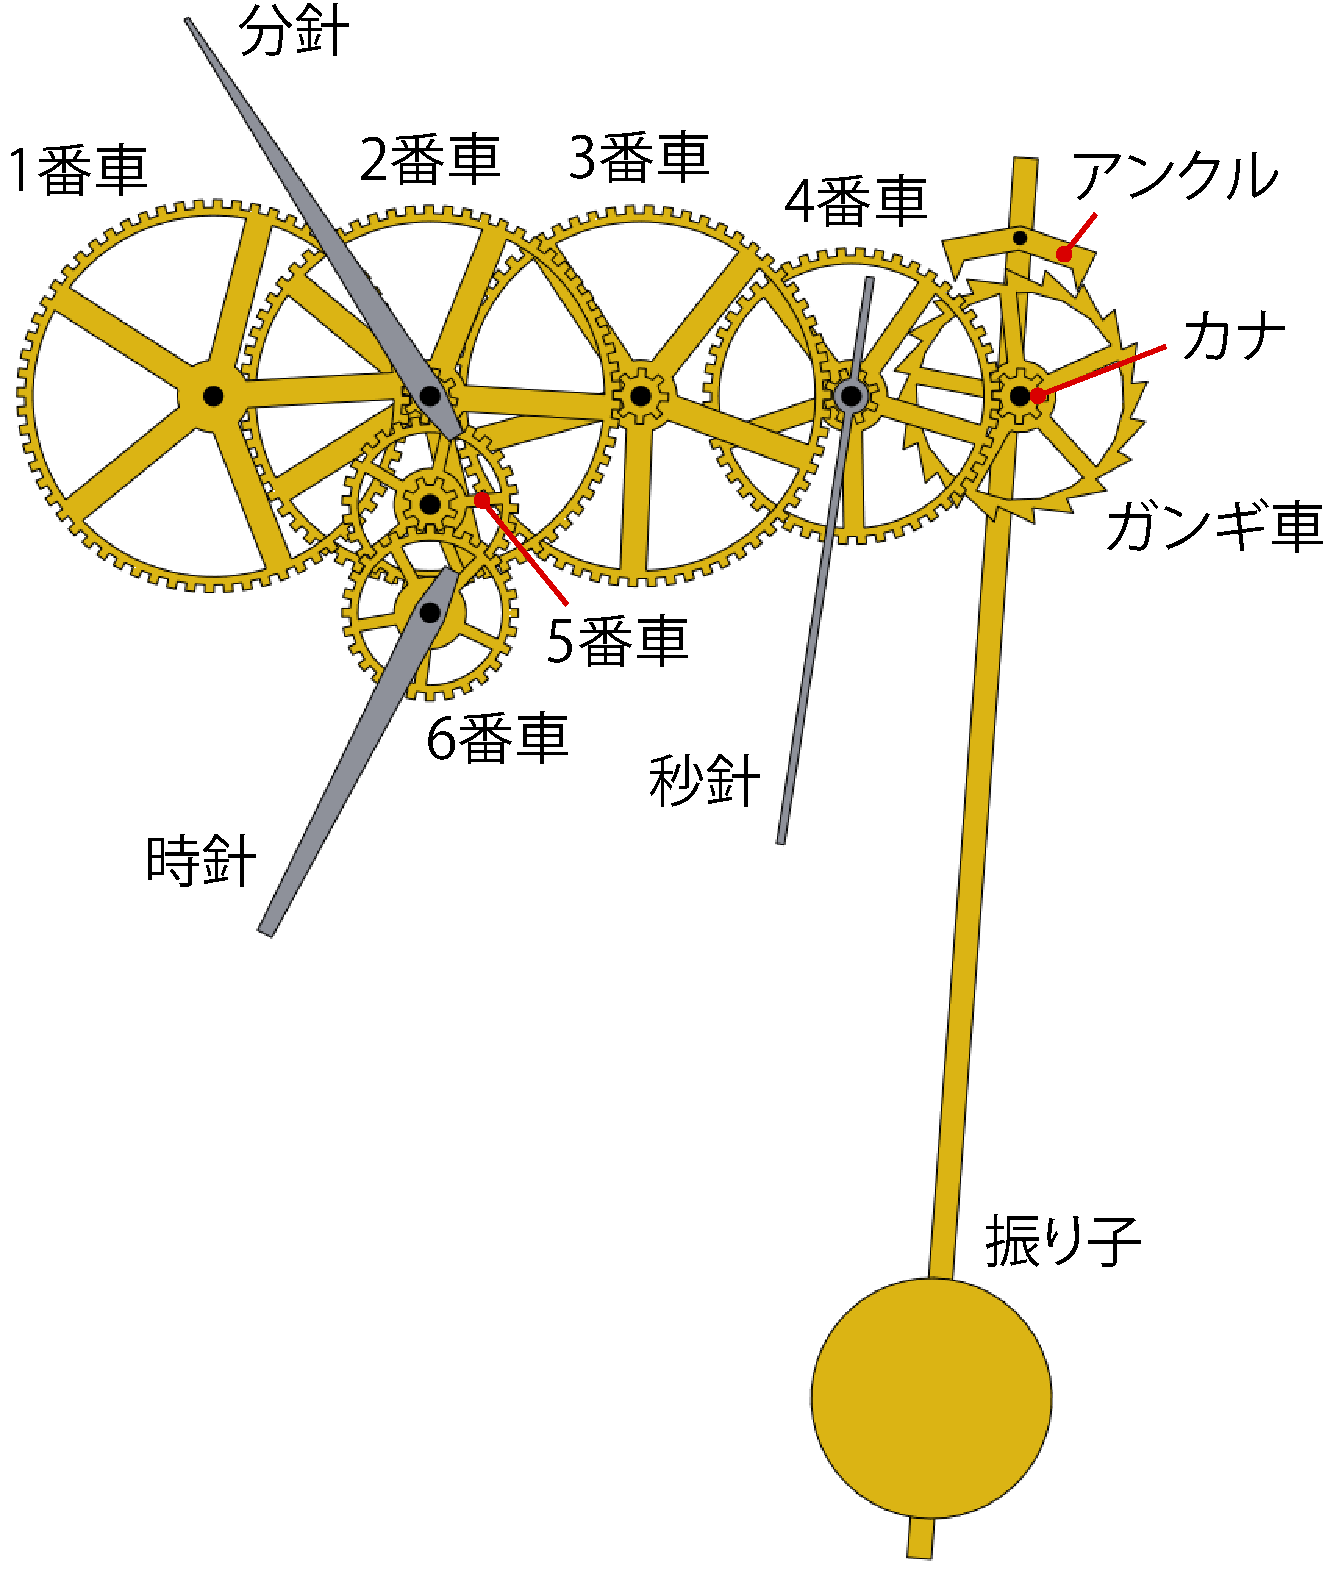
\includegraphics[width=10cm]{動作原理.pdf}
  \caption{振り子時計のパーツ}
  \label{fig:parts}
\end{figure}

図\ref{fig:parts}を見ると、1~6番車とガンギ車、アンクル、振り子で構成されていることが分かる。

2, 4, 6番車には、それぞれ分針、秒針、時針が取り付けられており、3, 5番車でそれぞれの回転速度の変換を行っている。
各歯車と、その中心にあるカナという歯車の歯数の比が、回転速度の比になる。
1番車は動力源となる歯車で、多くの場合は錘やモーター等によって動かされる。

しかしこれらのパーツだけでは、不安定な速度で周ってしまう。そこで、速度を一定に保つために振り子を利用する。
振り子には、振れ幅が十分小さければ、振れ幅に関係なく周期が一定になるという性質がある。
振り子の運動をガンギ車とアンクルで回転運動に変換することによって、精度良く回転速度を一定にすることができる。

なお、今回作成したプログラムでは、見栄えを良くするためにダミーの歯車を1つ追加した。これを0番車と呼ぶことにする。


\section{プログラムリスト}
プログラムのソースコードを、リスト\ref{lst:clock_h}--\ref{lst:shape_c}に示す。

\lstinputlisting[style=C,caption=clock.h,label=lst:clock_h]{clock/clock.h}

\lstinputlisting[style=C,caption=clock.c,label=lst:clock_c]{clock/clock.c}

\lstinputlisting[style=C,caption=shape.h,label=lst:shape_h]{clock/shape.h}

\lstinputlisting[style=C,caption=shape.c,label=lst:shape_c]{clock/shape.c}

\lstinputlisting[style=make,caption=Makefile,label=lst:make]{clock/Makefile}


\section{リソース}
プログラム中で用いられる文字盤の画像``dial.png''を図\ref{fig:dial}, アプリケーションのアイコン``icon.ico''を図\ref{fig:icon}に示す。

\begin{figure}[H]
  \centering
  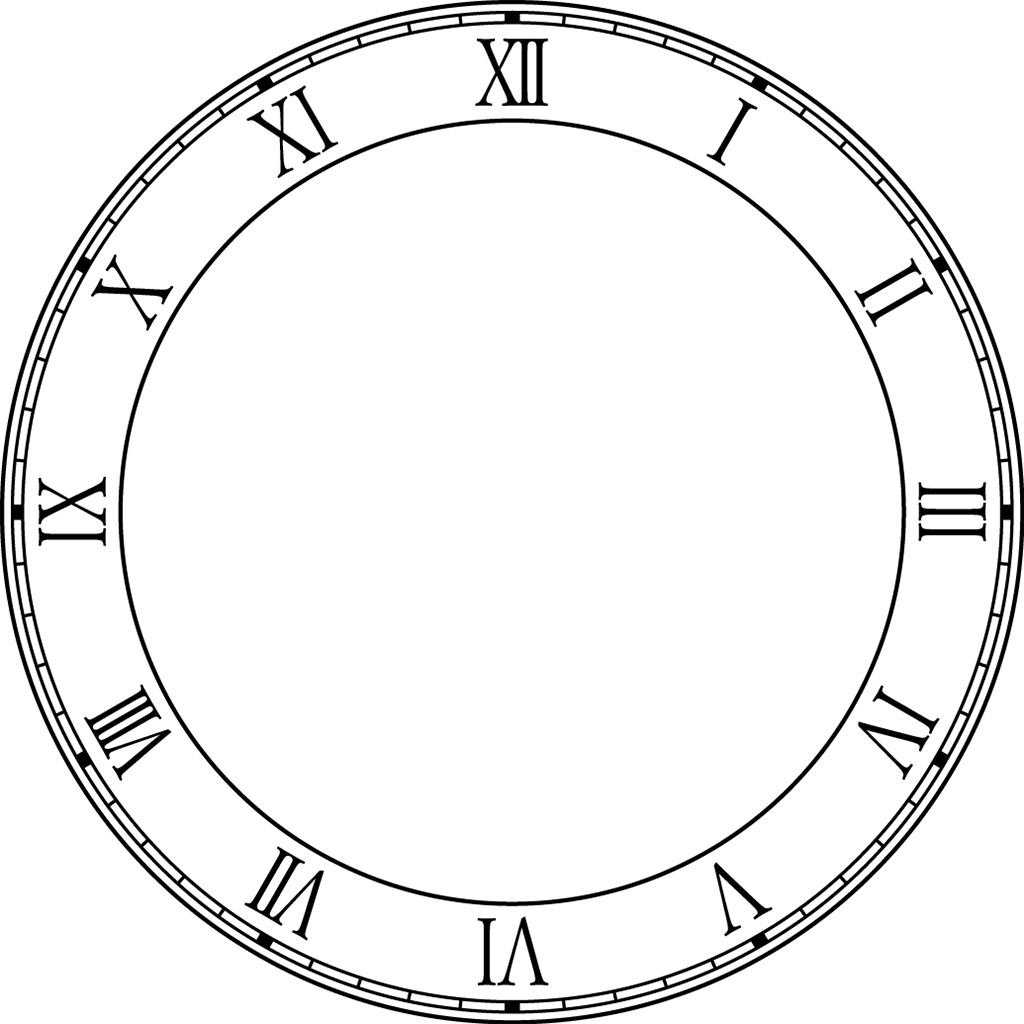
\includegraphics[width=8cm]{clock/dial.png}
  \caption{dial.png}
  \label{fig:dial}
\end{figure}

\begin{figure}[H]
  \centering
  
\includegraphics[width=4cm]{clock/icon-48.png}
  \caption{icon.ico}
  \label{fig:icon}
\end{figure}


\section{ビルド方法}
GLUTとglpngが導入されているCygwin上で、次のコマンドを入力することでビルド、実行することができる。

\begin{lstlisting}[style=text]
$ make
$ ./j16426.exe
\end{lstlisting}


\section{実行結果}
本プログラムを実行した結果を図\ref{fig:res1}に示す。
図\ref{fig:res1}を見ると、現在時刻が表示されており、文字盤の中には歯車と振り子が描画されていることが分かる。
また、振り子の動きに連動して各歯車と針が動いている。

\begin{figure}[H]
  \centering
  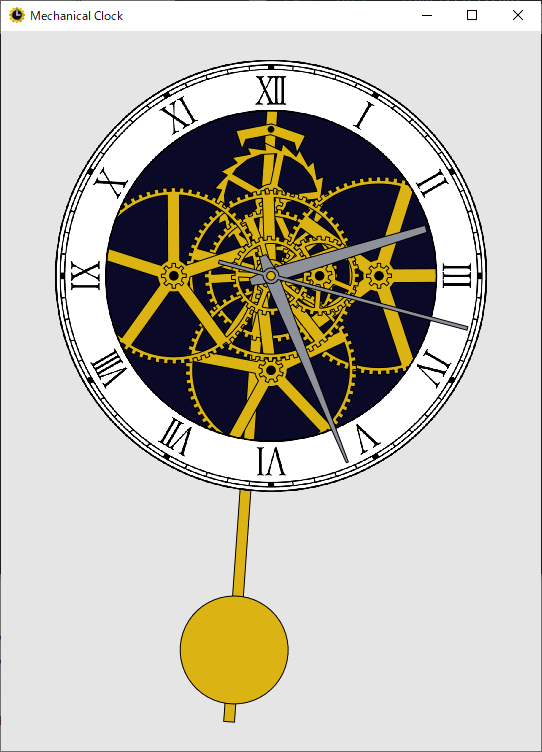
\includegraphics[width=7cm]{result1.png}
  \caption{実行結果}
  \label{fig:res1}
\end{figure}

\subsection{アニメーション}
アニメーションは、\texttt{glutTimerFunc}関数を用いて、短い間隔で描画関数を呼び出すことによって実現している。
タイマーのコールバック関数である\texttt{Timer}の中でさらにタイマーを登録することで、連続的なアニメーションを表現することが出来る。

また、\texttt{Timer}関数では現在時刻の取得も行う。
描画関数である\texttt{Display}の中で時刻の取得を行わないのは、機能ごとに関数を分けることで保守性や移植性などを高めるためである。

\subsection{座標系}
ウィンドウを横長になるように広げた状態を図\ref{fig:res2}, 縦長になるように縮めた状態を図\ref{fig:res3}に示す。
図\ref{fig:res2}を見ると、ウィンドウサイズに合わせて時計が拡大され、ウィンドウの中心に表示されている。
図\ref{fig:res3}を見ると、ウィンドウサイズを小さくしても見切れることなく、ウィンドウの横幅いっぱいに表示されていることが分かる。

\begin{figure}[H]
  \centering
  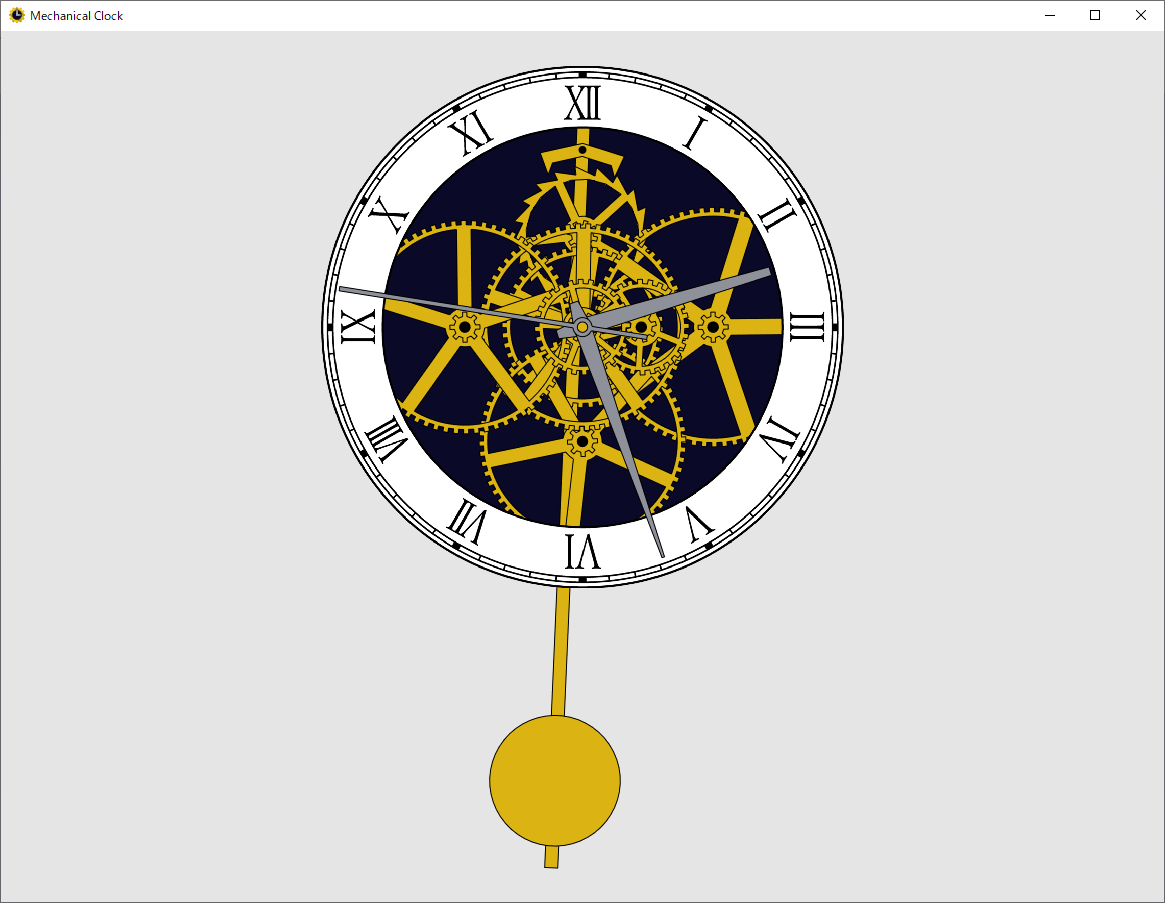
\includegraphics[width=15cm]{result2.png}
  \caption{横に長いウィンドウ}
  \label{fig:res2}
\end{figure}

\begin{figure}[H]
  \centering
  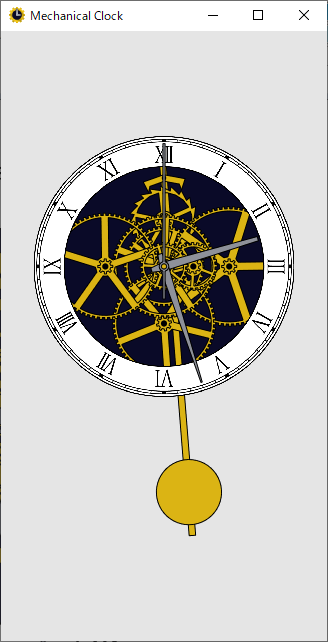
\includegraphics[width=4.25cm]{result3.png}
  \caption{縦に長いウィンドウ}
  \label{fig:res3}
\end{figure}

これは、ウィンドウサイズが変更された際に逐次座標系を変更しているためである。
ウィンドウが横に長い際の座標系は図\ref{fig:frame1}, 縦に長い際は図\ref{fig:frame2}のようになる。

\begin{figure}[H]
  \centering
  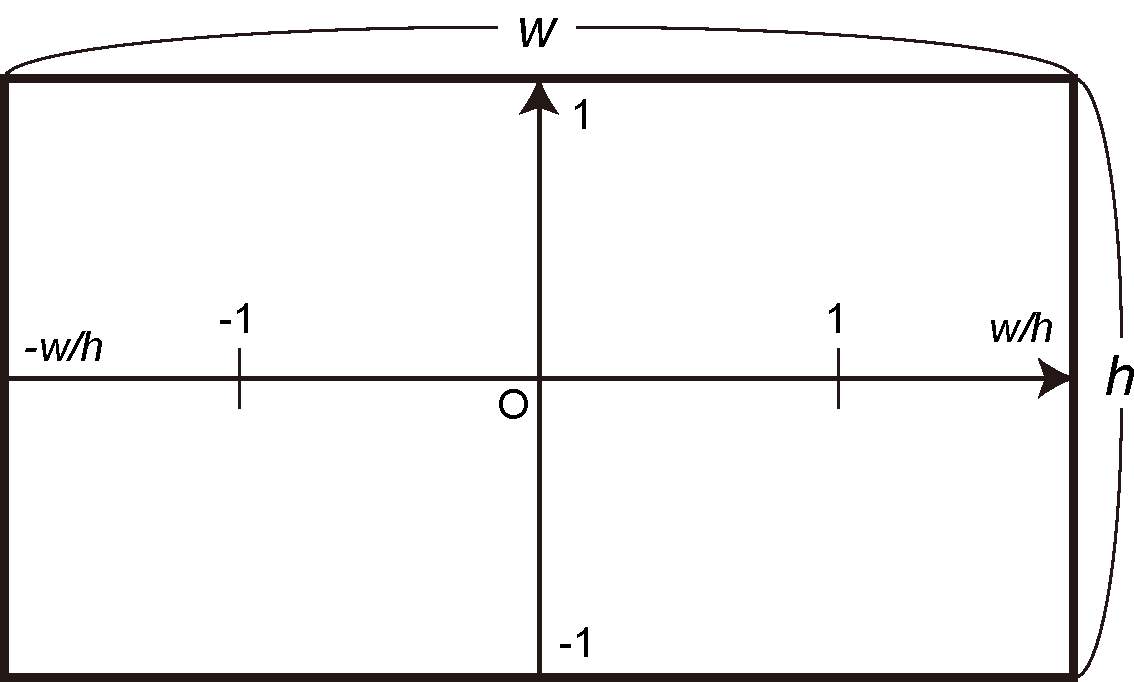
\includegraphics[width=10cm]{座標系1.pdf}
  \caption{横に長い座標系}
  \label{fig:frame1}
\end{figure}

\begin{figure}[H]
  \centering
  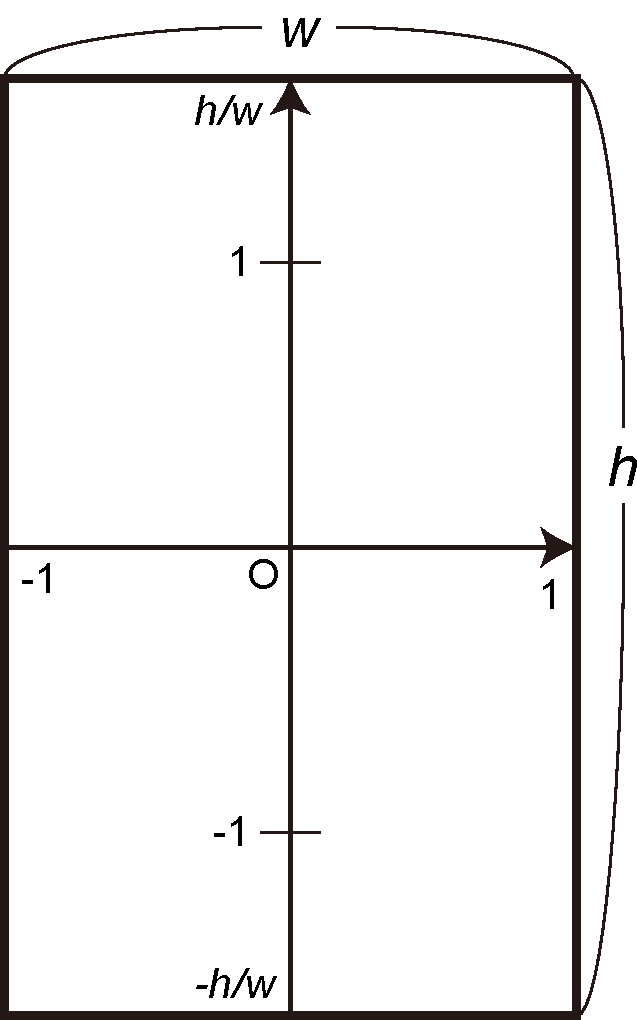
\includegraphics[width=6cm]{座標系2.pdf}
  \caption{縦に長い座標系}
  \label{fig:frame2}
\end{figure}

この設定を行っているのが\texttt{Reshape}関数である。ウィンドウサイズが変更された際に呼び出されるコールバック関数として\texttt{glutReshapeFunc}関数で登録されている。
\texttt{gluOrtho2D}という関数で画面端に対する座標を指定することができる。
これを図\ref{fig:frame1}, \ref{fig:frame2}のように設定することで、画面サイズに対する比で座標をしていすることになるので、
ウィンドウサイズが変更されてもそれに合わせて拡大縮小されるようになる。
また、$x$軸方向と$y$軸方向の座標の比を1:1になるようにしているため、横長、縦長にしても時計が潰れることなく、正円が保たれる。

\subsection{図形描画}


\begin{thebibliography}{9}
  \bibitem{bib:1} 伊藤祥一, ``Springs of C 楽しく身につくプログラミング'', 森北出版株式会社, 2017, pp. 109--110.
  \bibitem{bib:2} ``Pendulum clock'', Wikipedia, \texttt{\url{https://en.wikipedia.org/wiki/Pendulum_clock}}, 参照2019/12/5.
\end{thebibliography}


\end{document}
